%!TEX ROOT=ctutest.tex

%% Na obrazku lze videt xx obrazek ukazuje
%% trpny rod

\chapter{Softwarová implementace}
    Tato kapitola popisuje použité softwarové nástroje, chování celého systému a jednotlivých částí komunikačního řetězce.

\section{Architektura a chování celého systému}
    
    \subsection{Komunikační řetězec}
    V rámci správného fungování je důležité, aby spolu spolehlivě komunikovaly všechny tři části systému – měřicí jednotka (LoRa Node), centrální jednotka (LoRa Gateway) a aplikační server.
    Pro rádiovou komunikaci mezi měřicí jednotkou a bránou byl vytvořen binární komunikační protokol popsaný v~kapitole \ref{section:protokol}. Pro komunikaci brány a aplikačního serveru přes UDP soket byl vytvořen jednodušší komunikační textový protokol využívající formát JSON.\\
    Celkové chování systému nejlépe popisuje obrázek \ref{figure:app}, seznam všech rádiových paketů použitých v aplikaci diagram \ref{figure:radio_packets}.
    
    \subsubsection{Zahájení komunikace – Join proces}
    \label{section:join}
    Měřicí jednotka po stisknutí tlačítka reset začíná vysílat rádiový paket \texttt{Join Request}, čímž žádá nejbližší bránu o autorizaci. Jeho nejdůležitější informací je unikátní čtyřbajtový identifikátor uzlu – \textit{Unique Id} (na ST procesorech jako UUID uložený na specifické adrese), který má principiálně podobný účel jako MAC adresa, a časová známka RTC hodin. Jakmile do vypršení timeoutu neobdrží odpověď, opakuje jeho vysílání, dokud nepřijme rádiový paket \texttt{Join Reply}.\\
    Centrální jednotka po přijetí paketu vysílá do aplikačního serveru přes UDP soket požadavek \texttt{NodeInfo Request}. Pokud je dané zařízení registrované v databázi, dostává jako odpověď informace o měřicí jednotce, ve které se nachází uživatelem definovaná jednobajtová adresa jednotky – \textit{Session Id}, jež má podobný účel jako IP adresa a je využívaná po celý zbytek komunikace jako identifikátor jednotky. Dále se v odpovědi nachází komunikační port a jméno jednotky, a přihlášení je tak úspěšné.
    
    \subsubsection{Získání konfigurace – Configuration proces}
    \label{section:configuring}
    Po přijetí paketu \texttt{Join Reply} odesílá měřicí jednotka rádiový paket \texttt{Config Request}. Pokud po nejvýše třech neúspěšných odesláních nedostane odpověď, přechází opět do počátečního stavu po resetu.\\
    Centrální jednotka po přijetí paketu vysílá do aplikačního serveru přes UDP protokol požadavek \texttt{ConfigInfo Request}, na nějž dostává ze serveru odpověď v podobě konfigurace, kterou si uživatel vytvořil ve webovém rozhraní serveru a která byla uložena pro danou jednotku do databáze. Tato konfigurace je přeposlána do měřicí jednotky jako paket \texttt{Config Reply}.  Měřicí jednotka po jeho úspěšném přijetí ukládá konfiguraci do paměti a nastavuje podle ní příslušné periferie (rádiový modul, AD převodník, parametry FFT\ldots) (více v kapitole \ref{section:periferie}).
    
    \begin{figure}[!ht]
        \centering
	    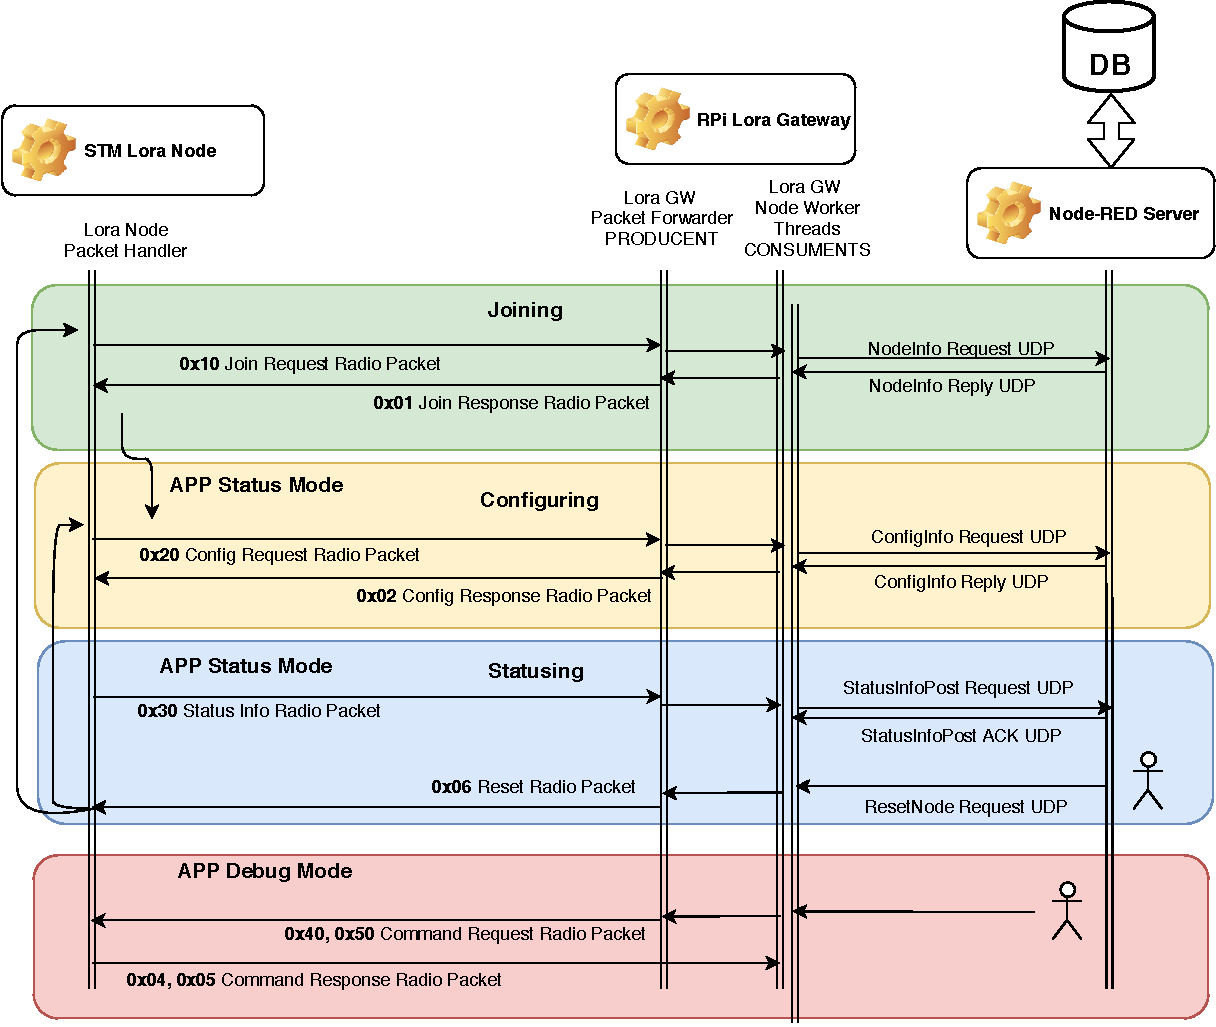
\includegraphics[width =1.1\textwidth]{SW_PART/Figs/app.pdf}
        \caption {Vizualizace chování celého systému. Hexadecimální čísla označují parametr \textit{CMD}.}
        \label{figure:app}
    \end{figure}  
    
    \subsubsection{Výsledky měření – Status proces}
    Jedním z nejdůležitějších parametrů konfigurace je údaj \textit{Stusinfo Interval}, jehož hodnota určuje, po jak dlouhém časovém intervalu vystoupí jednotka z~režimu spánku a odešle rádiový paket \texttt{Statusinfo} s naměřenými hodnotami baterie, teploty a s výsledky provedených analýz vibračního signálu z akcelerometru (popsáno v kapitole \ref{section:techniky}). Po přijetí paketu centrální jednotkou je jeho obsah upraven (převedení hodnot, doplnění o dodatečné informace) a data jsou přeposlána do aplikačního serveru, který je uloží do databáze.
    
    \subsubsection{Restart}
    \label{section:restart}
    Koncový uživatel má možnost interaktivně měnit konfiguraci měřicí jednotky v uživatelském rozhraní nebo danou jednotku restartovat. Konfigurace, kterou může uživatel nastavit, lze vidět v tabulce \ref{table:config}.\\
    Po stisknutí tlačítka ve webovém rozhraní je z aplikačního serveru do centrální jednotky odeslán přes UDP protokol požadavek na restart, který je po přijetí následujícího \texttt{Statusinfo} paketu přeposlán jako rádiový paket \texttt{Restart} do příslušné měřicí jednotky. Interval, po který měřicí jednotka naslouchá po odeslání \texttt{Statusinfo} paketu, je dán konfiguračním parametrem \textit{Statusinfo Listen Interval}.
    Podle jednobajtového těla paketu se poté rozhoduje, zda se vrátí do stavu, kdy žádá o konfiguraci, nebo přechází do stavu po stisknutí reset tlačítka (viz diagram \ref{figure:app}).
  
    
    \subsection{Rádiový komunikační protokol}
    \label{section:protokol}
    Pro účely komunikace mezi měřicí jednotkou a bránou byl navržen komunikační protokol, který slouží k rozlišení funkcionality jednotlivých paketů, přehlednou práci s přijatými nebo odesílanými daty a také pro jednoduché budoucí rozšíření celého systému o další pakety a další funkcionalitu.\\
    Při návrhu protokolu byl kladen důraz zejména na minimální možnou velikost paketů. Každý odeslaný bajt stojí měřicí jednotku energii z baterie. Vysílání je energeticky nejnáročnější úkon, který jednotka provádí (jednotlivé spotřeby v kapitole \ref{table:currents}), a proto byly například hodnoty RMS nebo teploty odesílány jako dvoubajtový integer namísto čtyřbajtového float, adresa měřicí jednotky je jednobajtová nebo hodnoty SF, šířky pásma a Coding Rate jsou odesílány jako jednobajtové údaje namísto konkrétních hodnot (jedná se v~podstatě o výčtové typy). Tyto hodnoty jsou upravovány do příslušné podoby až v~centrální jednotce.
    
    Každý radiopaket má pevně danou dvoubajtovou hlavičku, jež obsahuje parametr \textit{CMD} determinující význam paketu, a parametr \textit{sessionId} specifikující, komu je paket určen.
    Ve zbytku zprávy se nacházejí vlastní data paketu, jejichž velikost a obsah se liší podle konkrétního typu paketu, což je podrobně znázorněno na obrázku \ref{figure:radio_packets}.\\
    Komunikační protokol je implementovaný na straně brány v souboru\\ \texttt{radio\_packet.py} a na straně uzlu \texttt{radio\_protocol.h}.
    
 
    
 
\subsection{Konfigurace}
\label{section:config}
    Konfigurace měřicí jednotky může být uživatelem změněna ve webovém rozhraní (obrázek \ref{figure:gui_config}), jinak jsou vždy použité výchozí parametry. Výsledná konfigurace se poté nahrává do měřicí jednotky prostřednictvím rádiového paketu \texttt{Config Reply}. Seznam nejdůležitějších nastavitelných parametrů odpovídající záznamům v databázi lze vidět v následující tabulce.\\
    Díky navrženému datovému modelu (popsáno v \ref{section:data_model}) lze každé jednotce přiřadit jinou konfiguraci a také vymýšlet nová nastavení, a tím rozšiřovat celý systém. 
   
    \begin{table}[H]
        \begin{ctucolortab}
        \begin{tabular}{c!{\vrule width 2pt}c!{\vrule width 2pt}c}
            \textbf{Code} &  \textbf{Data Type} &  \textbf{Default Value} \\ 
            \Xhline{4\arrayrulewidth}
            adc\_samplings & text & 160CYCLES5 \\
            \hline
            adc\_divider & text & ASYNC\_DIV4 \\
            \hline
            fft\_samples\_num  & text & N\_1024\\ 
            \hline
            fft\_peaks\_num  & int & 5 \\ 
           \hline
            fft\_peaks\_delta  & int & 3 \\ 
           \hline
            lora\_codingrate  & text & CR4\_5 \\ 
           \hline
            lora\_spreadingfactor  & text & SF12 \\ 
            \hline
            lora\_bandwidth  & text & BW7\_8 \\ 
            \hline
            statusinfo\_interval  & int & 60 \\ 
            \hline
            statusinfo\_listen\_interval  & int & 5\\ 
            \hline
            dsp\_threshold\_voltage & float & 2.0\\ 
            \hline
            dsp\_rms\_averaging\_num & int & 1\\ 
            \hline
            dsp\_kurtosis\_trimmed\_samples & int & 10\\
        \end{tabular}
        \end{ctucolortab}
        \caption{Nejvýznamnější konfigurovatelná nastavení.}
        \label{table:config}
    \end{table}


\section{Měřící jednotka (LoRa Node)}
\subsection{Použité softwarové nástroje}

    Software měřicí jednotky byl vytvořen v programovacím jazyce C za použití vývojového prostředí Atollic TrueSTUDIO.\\
    Projekt byl založený na balíku dodaném firmou ST pro vývoj aplikací využívající síť LoRa – I-CUBE-LRWAN Expansion Package \cite{software:2}.\\ 
    Z tohoto balíku byly využity zejména knihovny pro obsluhu RF LoRa čipů SX1272/SX1276, inicializace některých periferií a dodatečné nástroje jako třeba logování na konzoli.
    Implementace linkové (MAC) vrstvy LoRaWAN protokolu využita nebyla z důvodů popsaných v kapitole \ref{section:single_channel_gw}.
    Pro rychlý výpočet RMS a FFT byla použita knihovna DSP obsahující také softwarovou emulaci operací s desetinnou čárkou \cite{software:1}.
   
    \begin{figure} [!ht]
	    \centering
	    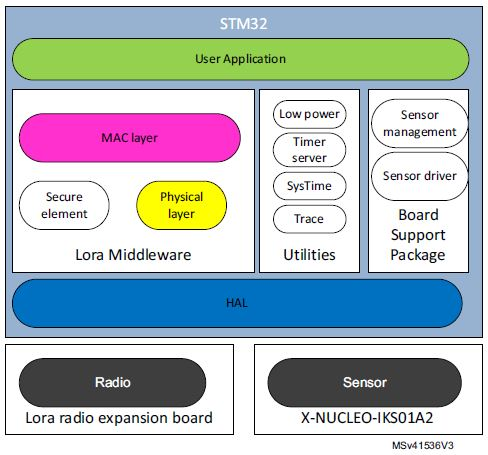
\includegraphics[ width = 0.5\textwidth]{SW_PART/Figs/st_loraextension.jpg}
        \caption {Hierarchie SW nástrojů dodaných firmou ST. Převzato z \cite{software:2}.}
    \end{figure}  
    
\subsection{Nastavení periférií a vzorkování}
\label{section:periferie}
  
    Po restartování systému jsou nastavené nejdůležitější periferie.
    Systémové hodiny monitorovací jednotky běží za pomocí PLL na dvojnásobné hodnotě frekvence HSI oscilátoru – 32 MHz, RTC hodiny na 32 kHz. Pro komunikaci s rádiovým modulem je nastavena SPI sběrnice s rychlostí 10 MHz, pro teplotní senzor $\text{I}^2\text{C}$ sběrnice s rychlostí 400 kHz, pro komunikaci s PC UART s rychlostí 115200 Bd/s, 8 datovými bity, 1 stop bitem a bez paritního bitu. Hodiny AD převodníku jsou odvozeny od HSI (v první verzi u Nuclea od HSE) oscilátoru a běží na 16 MHz.\\
    \begin{table}[!hbp]
    	\begin{ctucolortab}
    	     \begin{tabular}{c!{\vrule width 2pt}c}
                \textbf{Parametr} &  \textbf{Základní nastavení} \\ 
                \Xhline{4\arrayrulewidth}
    			Spreading Factor & 12 \\ \hline
    			Bandwidth & 125 kHz \\ \hline
    			Coding Rate & 4/5 \\ \hline
    			Frekvenční kanál & 868.5 MHz \\ \hline
    			Vysílací výkon & 5 dBm (PA\_BOOST) \\ \hline
                LNA &  0 dBm (maximum gain)\\ \hline
                Explicit header & OFF\\ \hline
                Low Data Rate Optimize & ON\\ \hline
                FHSS & OFF
    		\end{tabular}
    	\end{ctucolortab}
    	\caption{Základní TxRx nastavení LoRa modulu.}
    	\label{table:txrx}
    \end{table}
    
    Následně dochází ke konfiguraci LoRa modulu, kdy je pro každou měřicí jednotku nejprve použito základní nastavení (popsáno v tabulce \ref{table:txrx}).

    Vysílací výkon byl snížen na 5 dBm kvůli šetření baterie, pro kilometrové vzdálenosti by musel být zvýšen (spotřeba popsána v kapitole \ref{table:currents}). LNA (Low Noise Amplifier) byl nastaven na maximální zesílení, čímž bylo docíleno maximální citlivosti. SF byl použit vyšší – 12, což umožňuje vyšší selektivitu za cenu menší přenosové rychlosti.\\
    K dalšímu nastavení periferií dochází po přijetí rádiového paketu \texttt{Config Reply}. Konfigurace je nejprve uložena a dále je podle ní znovu nastaven LoRa modul a AD převodník.
    
    Pro přenos dat z akcelerometru slouží AD převodník zabudovaný přímo na čipu procesoru. Pro snadné řízení vzorkování byl využit DMA přenos, jenž přenáší navzorkovaná data z AD převodníku rovnou do paměti bez účasti procesoru. Výhoda DMA přenosu spočívá především v jeho rychlosti a přesném vzorkování.\\
    Vzorkovací frekvence AD převodníku je determinována konfigurací, konkrétně parametry \texttt{adc\_clock\_divider} a \texttt{adc\_sampling\_time} podle rovnice \ref{eq:fs}. Při jejím nastavování je třeba brát ohled na dodržení vzorkovacího teorému (popsáno v kapitole \ref{section:measuring}).
    
    \begin{equation}
        f_s = \frac{f_{HSI}}{clock\_divider}\,\frac{1}{(sampling\_time + 12.5)}
        \label{eq:fs}
    \end{equation}{}


\subsection{Měření a odeslání rádiového paketu Statusinfo}
   \begin{figure} [!hbp]
	    \centering
	    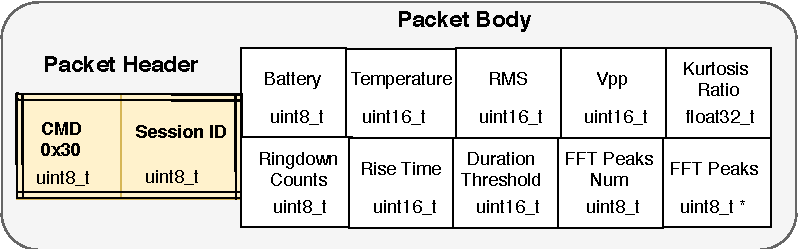
\includegraphics[ width =0.8\textwidth]{SW_PART/Figs/statusinfo.pdf}
        \caption {Struktura rádiového paketu Status Info.}
        \label{figure:statusinfo}
    \end{figure}  
    Po přijetí konfigurace je měřicí jednotka uspána a probuzena interruptem z RTC hodin. Doba, po kterou se nachází jednotka v režimu spánku je určena konfigurovatelným parametrem \texttt{statusinfo\_interval}. Nejprve dochází k~navzorkování dat z~akcelerometru, vyčtení dat z teplotního čidla, dále je naměřen stav baterie a následně dochází k preprocessingu signálu a vypočtení signálových analýz uvedených v kapitole \ref{section:techniky}. Data jsou poté odeslána jako rádiový paket \texttt{Statusinfo}, který, i přes snahu omezit jeho velikost, je nejdelším paketem ze všech rádiových paketů (viz \ref{figure:radio_packets}). Formát této zprávy lze vidět na obrázku \ref{figure:statusinfo} a jeho velikost je při základním nastavení 5 odesílaných maxim v amplitudovém spektru 49 bajtů.


%\subsection{Řízení spotřeby}
    


   
%%Softwarový vývoj postavený na platformě ST může probíhat několika odlišnými způsoby. Lze využívat knihovnu obsahující pouze registry procesoru – CMSIS, kterou dodává samotný ARM nebo nízkoúrovňové knihovny LL (Low Level) či již komplexní knihovny HAL (Hardware Abstraction Layer), jejichž dodavatelem je ST. Pro vývoj měřící jednotky byl pou nakonec použita kombinace p  Obsluha komunikace MCU přes UART byla například naprogramována pouze pomocí CMSIS, obsluha AD převodníku pomocí LL a obsluha I2C pomocí HAL.
 %%
 
\section{Řídicí jednotka (LoRa Gateway)}
\subsection{Použité softwarové nástroje}
    Na Raspberry Pi byl v první řadě nainstalován operační systém Raspbian  ve verzi bez grafického uživatelského rozhraní, který je založený na linuxovém Debianu a optimalizovaný pro Raspberry Pi. Pro samotný software centrální jednotky byl využit skriptovací programovací jazyk Python. Ten díky široké škále knihoven, které lze do projektu snadno importovat, usnadňuje vývojáři práci.\\
    Pro obsluhu GPIO pinů a periferií Raspberry jako SPI a UART byla využita knihovna \textit{wiringpi}.
    UDP komunikaci s Node-RED serverem zabezpečovala knihovna \textit{socket} a možnou HTTP komunikaci s RESTovým serverem knihovna \textit{requests}.
  
\subsection{Struktura aplikace – vícevláknový přístup}
    Z hlediska logické struktury byla aplikace rozdělena na hlavní vlákno a objekt reprezentující připojené měřicí jednotky tvořený 3 vlákny.\\
    Úkolem hlavního vlákna je neustálá a nepřerušovaná obsluha LoRa modulu – přijímání a odesílání paketů. Tato obsluha musí probíhat neustále a nesmí být závislá na jiných okolnostech zdržujících její průběh, jako je komunikace s Node-RED serverem či zpracovávání přijatých informací. Modul je nastaven v režimu kontinuálního příjmu, ze kterého může vystoupit pouze pokud je do odesílací fronty umístěn paket k odeslání.
    
    Objekt reprezentující měřicí jednotku je tvořen celkem třemi vlákny a obsahuje TX frontu pro UDP pakety na server, RX frontu dohromady pro přijaté UDP pakety ze serveru a rádiové pakety z měřicích jednotek a odkaz na TX frontu pro odesílané rádiové pakety (pro všechny jednotky společná). V~prvním vláknu \textit{worker} probíhá stavový automat aplikace, zpracování přijatých naměřených dat, jejich úprava, formátování do JSONu a logování. Zpracovaná data jsou prostřednictvím druhého vlákna \textit{sender} odesílána přes UDP soket do Node-RED serveru. Pro příjem dat z Node-RED serveru slouží třetí vlákno \textit{receiver}. 
    
    Vícevláknový přístup byl v centrální jednotce navržen zejména kvůli požadavku na neblokující řešení událostí. Aplikace po přijetí rádiového paketu z~měřicí jednotky, která na něj očekává odpověď, neblokuje komunikaci, dokud nejsou data přijata ze serveru, ale pokračuje v cyklu a zpracovávání dalších událostí. Příslušná odpověď na rádiovou zprávu ze serveru je nejprve přijata vláknem \textit{receiver} a následně umístěna do RX fronty, kterou kontroluje vlákno \textit{worker} a na kterou reaguje odesláním požadované rádiové odpovědi měřicí jednotce na základě přijatých informací ze serveru.\\
    Vícevláknový přístup také umožňuje řešit asynchronní události ze serveru, které přichází z webového rozhraní například při požadavcích na změnu konfigurace nebo restartování měřicích jednotek. 


\subsection{Řízení přístupu k rádiovému rozhraní}
    Jelikož centrální jednotka umožňuje komunikovat s více měřicími jednotkami, je třeba brát ohled na přístup k rádiovému rozhraní.\\
    V danou chvíli se totiž může stát, že jedna jednotka bude chtít odesílat informace o měření a druhá bude z brány přijímat konfiguraci.
    
    \begin{figure} [!h]
	    \centering
	    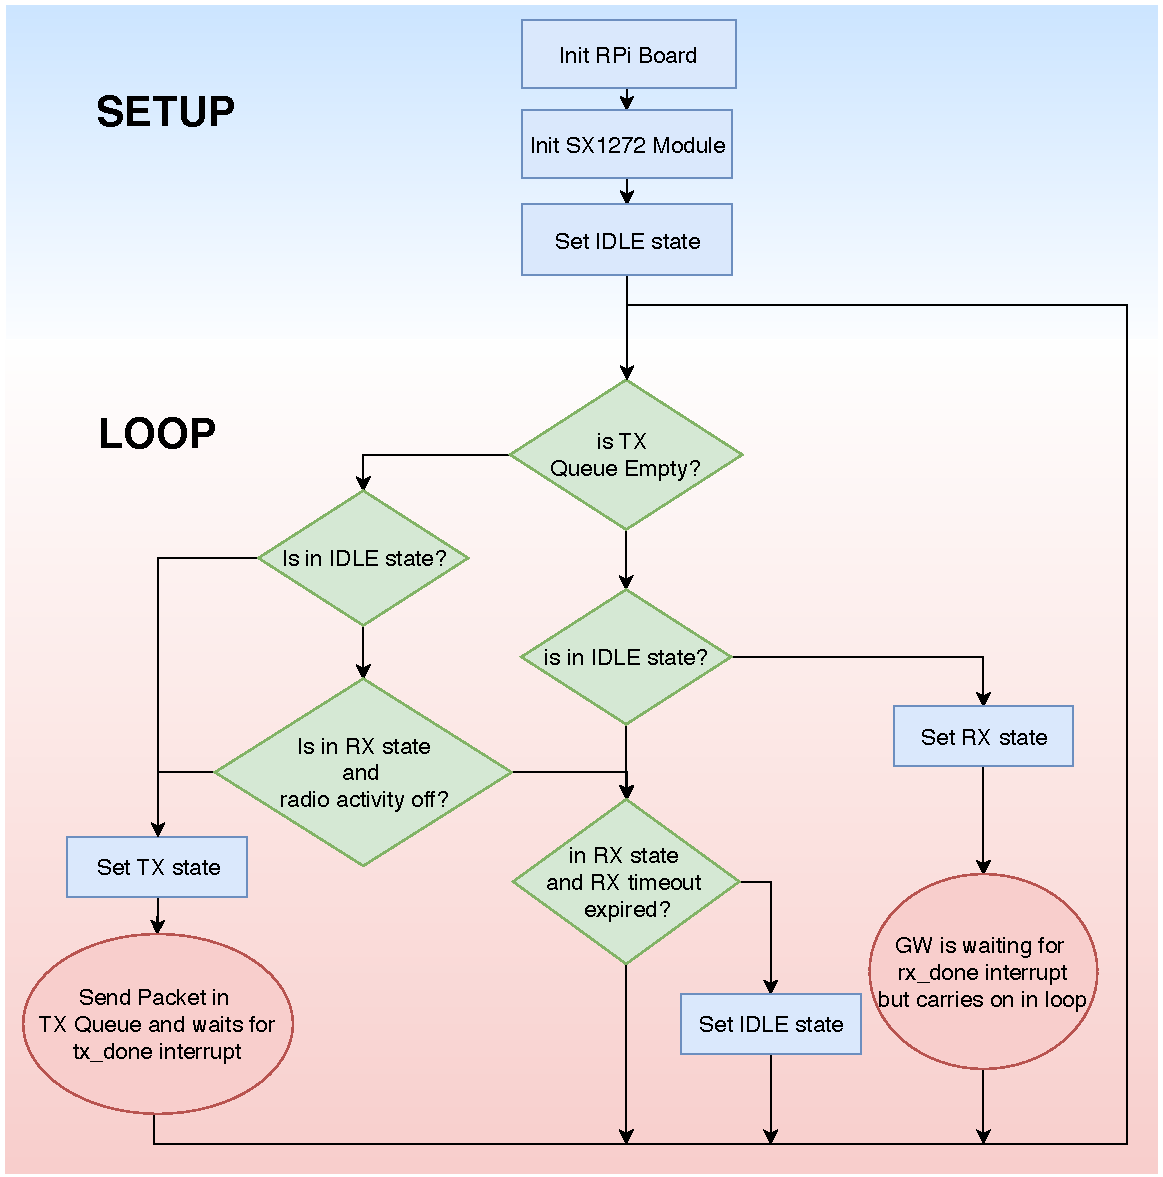
\includegraphics[ width =0.8\textwidth]{SW_PART/Figs/gw2.pdf}
        \caption {Hlavní smyčka obsluhující LoRa modul.}
        \label{figure:gateway_loop}
    \end{figure}  
    
    Zprávy ze všech komunikujících měřicích jednotek jsou přijaty v hlavním vlákně brány a to s nimi nakládá podle modelu producent-konzument. Přijatý paket tedy rozešle všem objektům reprezentujícím měřicí jednotky (umístí jej do RX front) a ty jej zpracují, pokud je pro ně paket určený (odpovídá parametr \textit{sessionId}).\\
    Zprávy, které potřebuje brána odeslat daným měřicím jednotkám, jsou nejprve vytvořeny v příslušném vláknu a přes společnou odesílací frontu jsou sdíleny s hlavním vláknem.
    
    Pro bránu je prioritní downlink – odesílání zpráv z brány. V hlavním cyklu se vždy kontroluje podmínka, zda je odesílací fronta prázdná. Pokud je prázdná, přechází brána do RX (přijímacího) módu, ve kterém setrvá až do vypršení timeoutu. Jakmile se tak stane a v odesílací frontě se objeví paket, je okamžitě odeslán a pokračuje se v cyklu (viz \ref{figure:gateway_loop}).
    

    
    
   
   
   
   
   
\section{Aplikační IoT server a databáze}
    Aplikační server a databáze jsou logicky odděleny od centrální jednotky na Raspberry a mohou být umístěny kdekoliv na internetu, což umožňuje větší modularitu celého systému. Ve vytvořené demo aplikace byly ale všechny části umístěny na Rapberry. Data s naměřenými hodnotami jsou po odeslání z centrální jednotky přes UDP soket umístěna do databáze. K vizualizaci slouží jednoduché uživatelské rozhraní, které data získává opětovnými SQL dotazy na databázi.
    
\subsection{Použité softwarové nástroje}
    Aplikační server byl vytvořen na platformě Node-RED \cite{website:6}. Tento nástroj, vyvíjený společností IBM, je postavený na javascriptovém serveru Node.js a uživateli umožňuje pohodlně propojovat hardwarová zařízení, APIs (aplikační rozhraní) a online služby za pomocí flowchartového programování a to vše ve webovém rozhraní. Uživatelské rozhraní bylo v Node-RED vytvořeno za pomocí doplňku \textit{node-red-dashboard} a komunikace s databází pomocí \textit{node-red-postgrestor}. Funkce pro obsluhu grafů, příjem a úpravu dat a ostatní logika serveru byla napsána v programovacím jazyce JavaScript.\\ 
    Pro ukládání dat byla využita opensourcová databáze PostgreSQL \cite{website:7}. Jedná se o relační databázi, kde jednotlivé klíče (unikátní identifikátory typu UUID) udávají vztahy mezi tabulkami a záznamy v databázi, což lze dobře vidět na datovém modelu aplikace na obrázku \ref{figure:data_model}. 


\subsection{Komunikace s řídící jednotkou}
    \begin{figure} [!h]
	    \centering
	    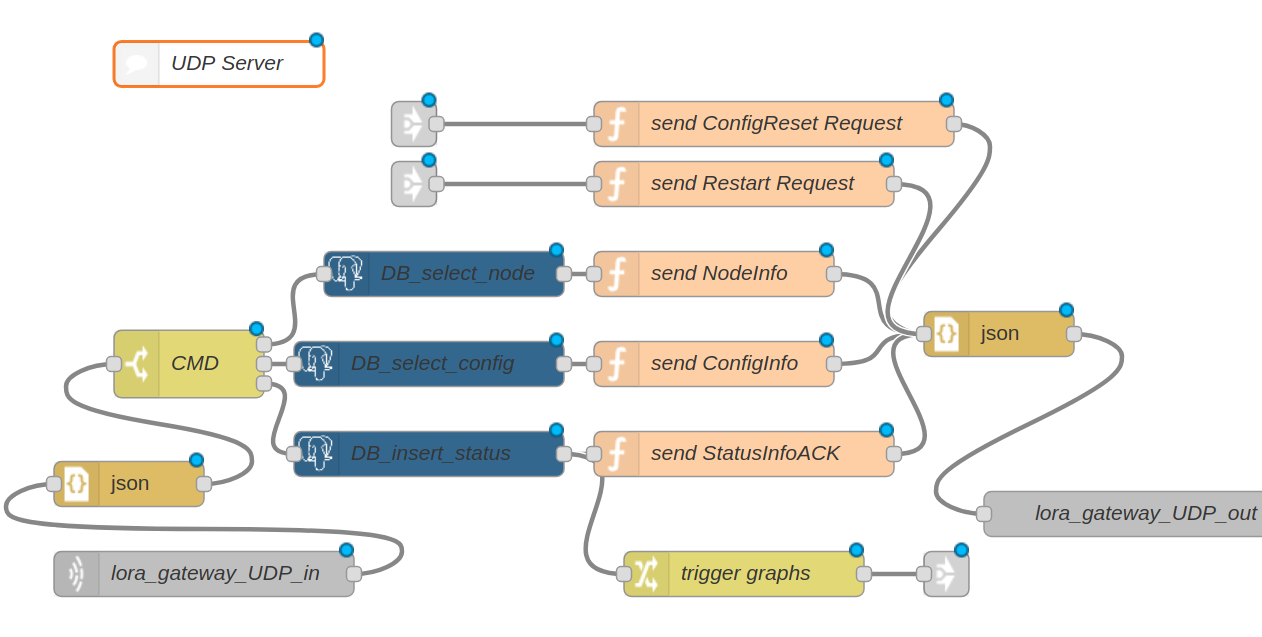
\includegraphics[ width =1.1\textwidth]{SW_PART/Figs/Node-RED/node_red_udp.png}
        \caption {Program pro obsluhu UDP soketu serveru.}
    \end{figure} 
    
    Centrální jednotka komunikuje z příslušných vláken reprezentujících měřicí jednotky se serverem prostřednictvím UDP soketu a textového protokolu ve formátu JSON. Veškeré dotazy na server jsou směřovány na port 8888 a jsou zpracovávány podle parametru \textit{CMD} definujícího typ požadavku a parametru \textit{idLoraNode} určujícího konkrétní jednotku. Odpověď je odesílaná na stejný port, ze kterého dotaz přišel. Jediný případ, kdy samotný server zasílá požadavek centrální jednotce, nastává při změně konfigurace jednotky nebo při jejím restartování a je směřován na port, který je pro příslušnou jednotku uložen v databázi.
    
    
    
\subsection{Komunikace s aplikacemi třetích stran – REST API}

    Krom řídící jednotky je server připraven poskytovat data i aplikacím třetích stran, k čemuž slouží rozhraní vybudované na základě REST-JSON. S tímto rozhraním pak může komunikovat jakákoli další klientská aplikace, tedy například webový interface, který data získává pomocí javascriptu, nebo další připojený systém, což umožňuje koncovému uživateli velikou flexibilitu a rozšiřuje možnosti využití systému.\\ 
    Data z databáze lze získat přes HTTP GET dotaz na url reprezentující jednotlivé tabulky v databázi (vypsané níže – \ref{code:url}), kde se v hlavičce dotazu specifikuje identifikační číslo – \textit{idLoraNode} daného uzlu. IP adresa serveru se liší podle toho, kde je server umístěn, port je standardní – 1880. Jako odpověď přichází záznamy z databáze ve formátu JSON. Pro přesnější výsledky je v~rozhraní systému umožněno SQL-like dotazování použitím základních SQL struktur (parametry WHERE, ORDERBY, LIMIT\ldots v těle GET dotazu).\\
    Data lze přes RESTové rozhraní do databáze také uměle přidávat přes POST dotaz na stejné url adresy jako v případě čtení dat.
    
    \begin{figure}[!hbp]
        \centering
        \begin{lstlisting}
        http://<Node-RED ip>:1880/lora_nodered/config
        http://<Node-RED ip>:1880/lora_nodered/nodeinfo
        http://<Node-RED ip>:1880/lora_nodered/statusinfo\end{lstlisting}
        \caption{Seznam URL adres namapované na údaje v databázi.}
        \label{code:url}
    \end{figure}{}
    \begin{figure} [!htp]
	    \centering
	    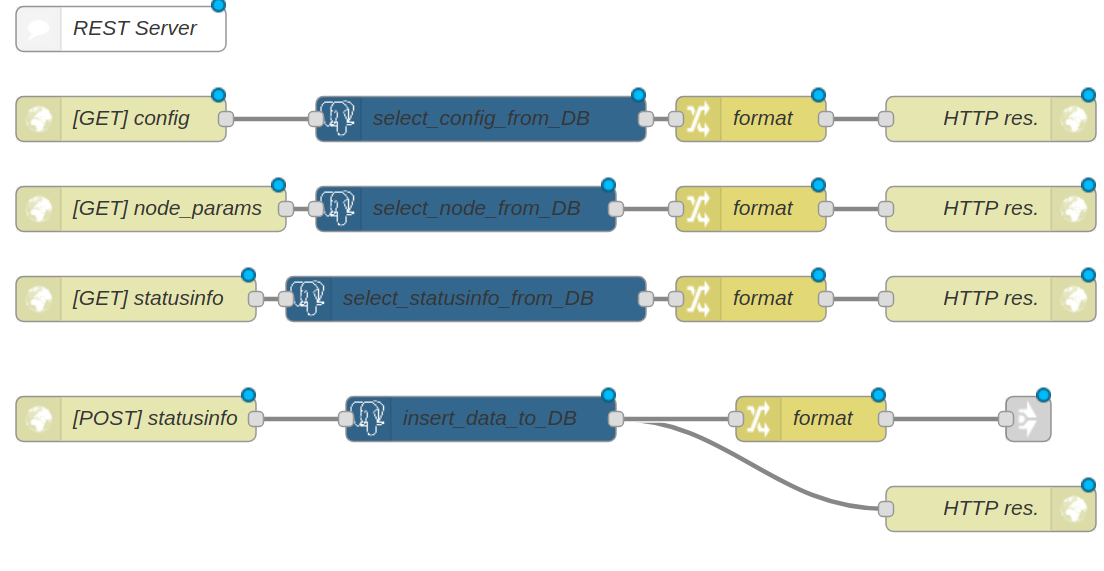
\includegraphics[ width =\textwidth]{SW_PART/Figs/Node-RED/node_red_rest.png}
        \caption {Program pro obsluhu RESTového serveru.}
    \end{figure} 
    
   
    

   
\subsection{Datový model}
\label{section:data_model}
    Pro účely aplikace byl vytvořen datový model, postavený na principech relačních databází, který je znázorněn na obrázku \ref{figure:data_model}. Databáze je tvořena celkem čtyřmi tabulkami, z nichž nejvýznamnější je \textit{StatusInfo}, ve které jsou uložená data z měření, a \textit{LoRaNode} s údaji o měřicích jednotkách.
    Tabulky \textit{Configuration} a \textit{ConfigurationValue} slouží pro vytvoření konfigurovatelných parametrů a jejich konkrétní hodnoty pro dané měřicí jednotky.
    
    \begin{figure}[!hbp]
        \centering
        \begin{lstlisting}
            SELECT "datatype", value, code 
                FROM app_configuration_value a 
                JOIN app_configuration b
                ON a.idsetting = b.idsetting
                WHERE idobjectrelated = '{{msg.payload}}';\end{lstlisting}
        \caption{Ukázka SQL query pro výběr konfigurace příslušné jednotky z~databáze.}
        \label{code:sql}
    \end{figure}
    \begin{figure} [!htp]
	    \centering
	    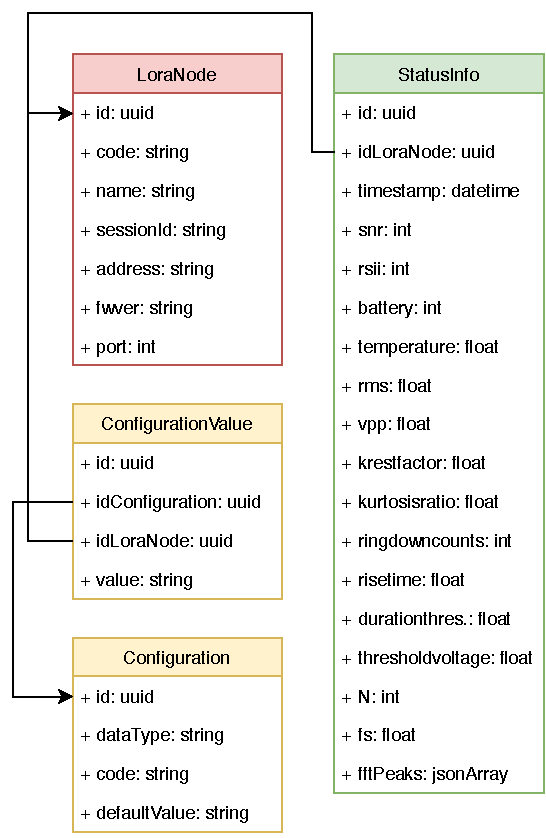
\includegraphics[ width = 0.55\textwidth]{SW_PART/Figs/data_model.pdf}
        \caption {UML diagram datového modelu aplikace.}
        \label{figure:data_model}
    \end{figure} 



    
\subsection{Uživatelské rozhraní}
\label{section:gui}
    V rámci serveru bylo vytvořeno také jednoduché uživatelské rozhraní. Po vybrání konkrétní jednotky ze seznamu, lze v druhém a třetím panelu (obrázky \ref{figure:experiment_graphs02} a \ref{figure:gui_other}) na příslušných grafech pozorovat časové změny monitorovaných veličin – teploty, RMS, stavu baterie, krest faktoru, nejvýznamnějších maxim v~amplitudovém frekvenčním spektru\ldots
    V prvním panelu se nachází dodatečné informace o RSSI, SNR a časové známce posledního přijatého paketu a formulář, v němž lze změnit konfiguraci jednotky, která se poté uloží po stisknutí tlačítka Load Config do databáze a pokud je jednotka připojena, dojde k jejímu resetování (viz. kapitola \ref{section:restart}). Pro vrácení jednotky do původního stavu slouží tlačítko Restart (viz obrázek \ref{figure:gui_config}). 
    
    \begin{sidewaysfigure}
        \centering
        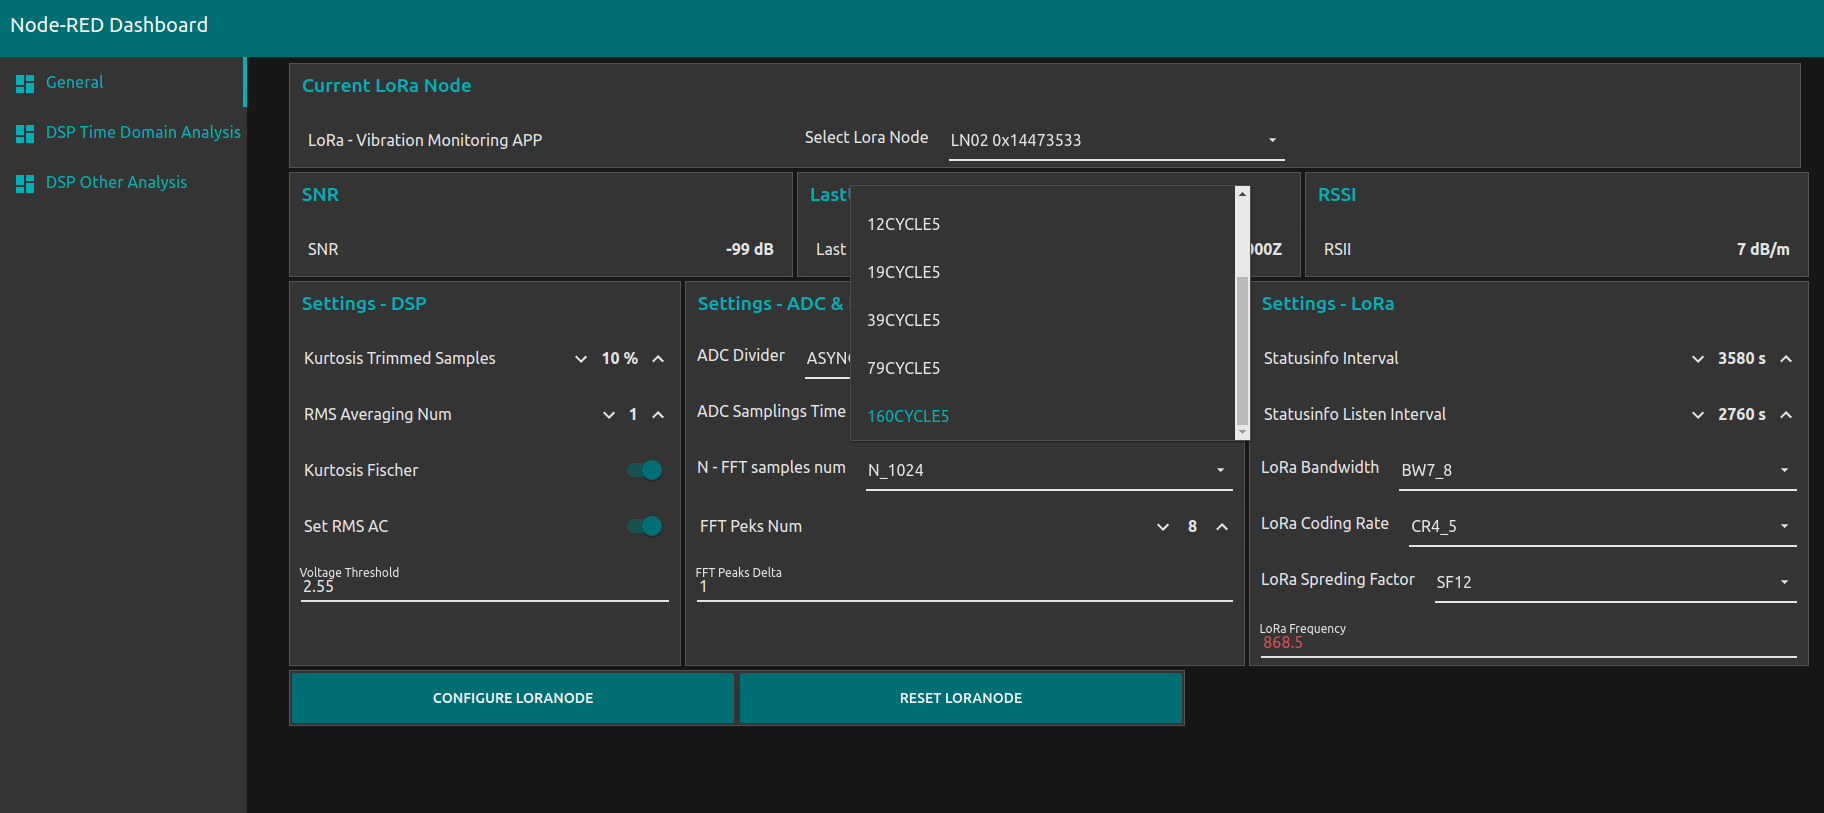
\includegraphics[ width =\textwidth]{SW_PART/Figs/gui_config.png}
        \caption {První panel uživatelského rozhraní pro nahrání konfigurace.}
        \label{figure:gui_config}
    \end{sidewaysfigure}
    
        
    \begin{sidewaysfigure}
        \centering
        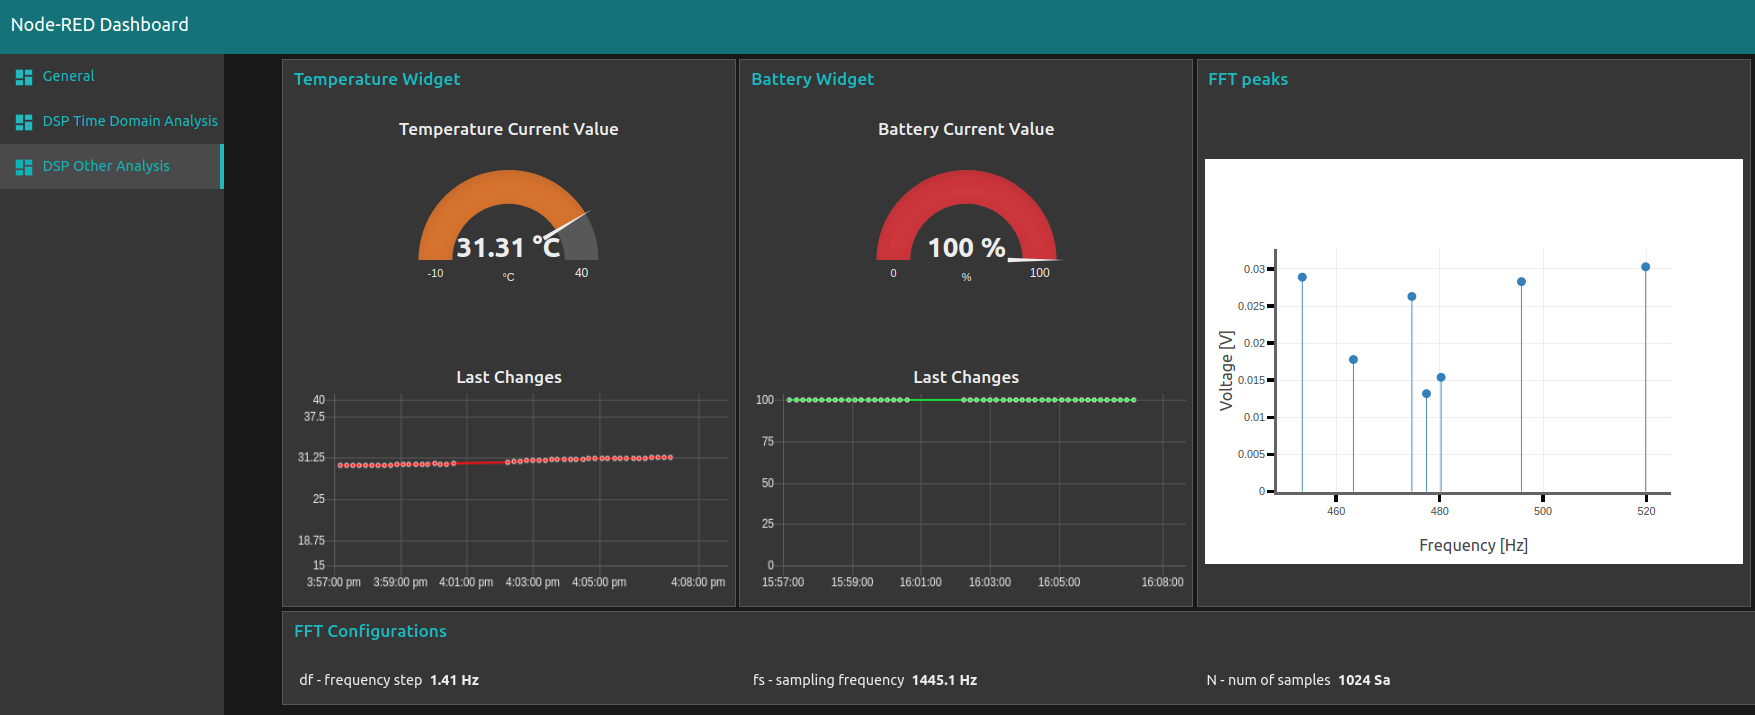
\includegraphics[ width =\textwidth]{SW_PART/Figs/gui_other.png}
        \caption {Druhý panel uživatelského rozhraní.}
        \label{figure:gui_other}
    \end{sidewaysfigure}

    

    
    